Chimera states in brain models have often been linked loosely to
unihemispheric sleep,
seizures,
and other brain behaviors \cite{Abrams2008,Panaggio2015,Martens2013,Abrams2004,Shanahan2010,Hohlein2019,Bansal2019,Chouzouris2018}.
In most cases,
these connections are made in off-hand remarks to introduce the concept of a chimera state,
but serious connections between these phenomena are rarely drawn.
However,
there are some notable cases of investigations of chimera states in brains.

\subsubsection{Square Torus}
\label{sec:lit_review_chimera_square_torus}
One such example is an investigation of two different neural models
(FitzHugh-Nagumo neurons and leaky integrate-and-fire neurons, both known to be accurate neural models \cite{Deco2008})
run on a toroidal square network of $N \times N$ nonlocally coupled neurons \cite{Schmidt2017}.
The most important result of this simulation is that similar behaviors appeared in each.
It was found that FitzHugh-Nagumo and leaky integrate-and-fire neurons not only can produce chimera states,
but produce chimera states in similar shapes and patterns.

For example,
both types of neurons produced isolated disks of high synchrony while the rest of the torus was oscillating asynchronously (coherent-spot),
as well as disks of asynchrony while the rest of the system was oscillating synchronously (incoherent-spot).
Both types of neurons also produced states in which a ring of neurons were firing synchronously
between two areas of asynchronous oscillation (coherent-ring),
and vice versa (incoherent-ring).

This similar behavior indicates that the presence of chimera states is not simply a function of the precise model chosen,
but a quality universal to brain activity.
Thus, it makes sense to postulate that chimera states will appear in any reasonably accurate brain model.
The main caveat for that takeaway is that the network topology chosen for these models was not necessarily representative of the topology of an actual brain (see \cref{sec:methods_network}).
However, seeing as the models both presented chimera-like behavior,
these states are well worth pursuing in other models.

\subsubsection{Chimera Collapse}
\label{sec:lit_review_chimera_collapse}
Chimera states are transient behavior for finite networks of oscillators \cite{Wolfrum2011}.
This means that a finite number of oscillators will eventually collapse into a totally synchronous state.
This transition occurs suddenly, but does provide warning signs.
As the system gets closer to collapse, the asynchronous group gets increasingly incoherent \cite{Andrzejak2016}.
This is counterintuitive, as the asynchronous group is already almost incoherent (by definition).
However, the order parameter of an asynchronous group is rarely 0.
As an example, in the snapshot of the simulation of the Kuramoto model (\cref{fig:kuramoto_snapshot}), the asynchronous group is generally gathered around $\phi = -\frac{\pi}{2}$.
The asynchronous group's non-zero coherence provides it its own mean-field (however spread it may be), which protects it from being absorbed into the synchronous group.
Thus, when the coherence of the asynchronous group decreases, this mean-field goes away, leaving the asynchronous group susceptible to collapse.

This hypo-coherence preceding chimera state collapse was observed in transcranial EEG recordings of patients undergoing seizures \cite{Andrzejak2016}.
However, the authors were very clear that the analogies between chimera state collapse and seizures are extremely conceptual.
It has yet to be shown whether chimera state collapse specifically is related to seizure activity in any way.

\subsubsection{Chimeras in a Cat Model}
\label{sec:lit_review_chimera_cat}
A final example of a chimera state being investigated in neural models (and the inspiration for this work) was an exploration of chimera states on a network of Hindmarsh-Rose neurons (\cref{eq:hr_x,eq:hr_y,eq:hr_z}) \cite{Santos2017}.
This model was simulated on the connectome of a cat (\cref{fig:cat_matrix}).
\begin{figure}[ht]
  \centering
  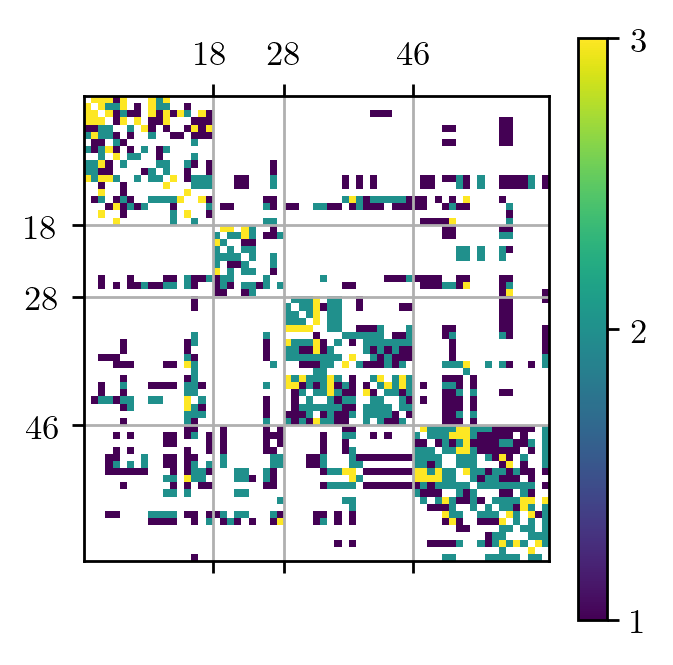
\includegraphics[width=0.9\columnwidth]{figure/cat_matrix}
  \caption[Cat connectome]{The cat connectome, represented as a matrix.
    The cat brain was divided into 4 cortices (visual, auditory, somato-motor, and frontolimbic) with 65 subcortices.
    The connection strength between the subcortices was measured and placed on a scale of 1, 2, or 3.
  }
  \label{fig:cat_matrix}
\end{figure}
Parameter space for the two connection strengths $\hra$ and $\hrb$ was explored.
Chimera states are most prevalent for low values of $\hrb$, the inter-cortex connection strength \cite{Santos2017}.
This is unsurprising.
If the inter-cortex connection strength is too high as compared to the intra-cortex connection strength, the coupling acts global instead of nonlocal.
This means that each cortex has less holding it together than pulling it apart, allowing the system to descend into asynchrony.

Additionally, with increasing input current $I_{0}$ (and increasing noise in the input current), chimera states give way to incoherence.
This also intuitively makes sense.
As the input current increases, its significance relative to the coupling also increases.
Thus, the oscillators have no reason to synchronize.
And, of course, adding noise will simply amplify the effect.
